\documentclass[pdf,ps,8pt]{beamer}

\usepackage{lmodern}
\usepackage{amsmath}
\usepackage{color}
\usepackage{bbold}
\usepackage{cancel}
\usepackage{slashed}
\usepackage{graphicx}
\usepackage{verbatim}
\usepackage{textcomp}

\usetheme{Singapore}

\definecolor{palegray}{rgb}{0.82,0.822,0.82}
\newcommand{\preliminary}{
{ \rput{30}(7,-4.0){\fontsize{40}{40}\selectfont {\color{palegray}Preliminary Preliminary}} }
}

\newcommand{\textapprox}{\raisebox{0.5ex}{\texttildelow}}

\newcommand{\miniscule}{\fontsize{3pt}{4pt}\selectfont}

\def\MSbar{$\overline{\mathrm{MS}}$}
\def\gev{\,\mathrm{GeV}}
\def\mev{\,\mathrm{MeV}}
\def\fm{\,\mathrm{fm}}
\def\SU{\mathrm{SU}}
\def\su#1#2{\SU(#1)_\mathrm{#2}}
\def\rpisq{\langle r_\pi^2\rangle}
% final values
\def\rpisqsim{0.38(4)}  % pole fit for 330 MeV pion
\def\rpisqsu2sim{0.354(31)}  % su2 fit for 330 MeV pion
\def\rpisqsimlong{0.382(42)}
\def\rpisqphys{0.418(31)} % SU(2) chi extrap
\def\rpisqphyslong{0.418(31)}
\def\lsixr{-0.0093(10)} % SU(2)
\def\Lniner{0.0031(6)}  % SU(3)

\newcommand{\chpt}{\chi^{\rm PT}}
\newcommand{\tchpt}{$\chi^{\rm PT}$}
\newcommand{\tchptthree}{$\chi^{\rm PT}_3$}
\newcommand{\tchpttwo}{$\chi^{\rm PT}_2$}

\newcommand{\xiav}{\langle\,\xi\,\rangle}
\newcommand{\xisqav}{\langle\,\xi^2\,\rangle}


\newcommand{\mD}{\left(\begin{array}{cc} \DO & \Dd \\  \Ddb&\DOb \end{array} \right)}

\newcommand{\Ob}{\bar{\Omega}}

\newcommand{\DO}{D_\Omega}
\newcommand{\Dd}{D_\partial}
\newcommand{\DOi}{D_\Omega^{-1}}
\newcommand{\DOid}{D_\Omega^{-\dagger}}
\newcommand{\Pd} {\mathbb{P}_\partial}
\newcommand{\PO} {\mathbb{P}_\Omega}

\newcommand{\DOb}{D_{\bar{\Omega}}}
\newcommand{\Ddb}{D_{\bar{\partial}}}
\newcommand{\DObi}{D_{\bar{\Omega}}^{-1}}
\newcommand{\DObid}{D_{\bar{\Omega}}^{-\dagger}}
\newcommand{\Pdb}{\mathbb{P}_{\bar{\partial}}}
\newcommand{\POb} {\mathbb{P}_{\bar\Omega}}

\newcommand{\Phidb}{\mathbb{\phi}_{\bar{\partial}}}
\newcommand{\etadb}{\mathbb{\eta}_{\bar{\partial}}}

\newcommand{\hDO}{\hat D_\Omega}
\newcommand{\hDd}{\hat D_\partial}
\newcommand{\hDOi}{\hat D_\Omega^{-1}}
\newcommand{\hPd} {\hat{\mathbb{P}}_\partial}

\newcommand{\hDOb}{\hat D_{\bar{\Omega}}}
\newcommand{\hDdb}{\hat D_{\bar{\partial}}}
\newcommand{\hDObi}{\hat D_{\bar{\Omega}}^{-1}}
\newcommand{\hPdb}{\hat{\mathbb{P}}_{\bar{\partial}}}

\newcommand{\mul}[1]{\left(\begin{array}{cc}#1 & 0 \\ 0& 0\end{array}\right)}
\newcommand{\mur}[1]{\left(\begin{array}{cc}0  & #1\\ 0& 0\end{array}\right)}
\newcommand{\mll}[1]{\left(\begin{array}{cc}0  & 0 \\ #1 & 0\end{array}\right)}
\newcommand{\mlr}[1]{\left(\begin{array}{cc}0  & 0 \\ 0& #1\end{array}\right)}

\newcommand{\mDO}{\mul{ \DO}}
\newcommand{\mDd}{\mur{ \Dd}}
\newcommand{\mDOi}{\mul{\DOi}}
\newcommand{\mPd} {\mlr{\Pd}}

\newcommand{\mDOb}{\mlr{\DOb}}
\newcommand{\mDdb}{\mll{\Ddb}}
\newcommand{\mDObi}{\mlr{\DObi}}
\newcommand{\mPdb}{\mul{\Pdb}}
\newcommand{\rmod}{\mathrm{mod}}
\newcommand{\rdiv}{\mathrm{div}}

\newcommand{\link}[1]{\href{#1}{ {\color{blue} #1} }}

\beamertemplatenavigationsymbolsempty
\begin{document}



\begin{frame}[fragile]\small\frametitle{  Computational Methods (practice) -  Lecture 3    }

  \begin{center}
 
  {\color{red} Peter Boyle} (BNL, Edinburgh)

  \begin{itemize}
  \item Krylov methods and approximate matrix inversion
  \item GMRES
  \item Conjugate Gradients
  \item Preconditioning
  \item Red black preconditioning
  \item Checkerboarded implementation
  \item Multigrid preconditioning
  \item Eigensolvers and Deflation
  \end{itemize}

\end{center}  
\end{frame}

  \begin{frame}[fragile]\small\frametitle{ Krylov methods and approximate matrix inversion}
  \begin{itemize}
  \item Algorithms minimise a residual $|r|^2$, where
    $$
    r = M \psi - b
    $$
  \begin{itemize}
  \item $r=0 \Leftrightarrow \psi = M^{-1} b$ so minimise $r$ under some norm
  \end{itemize}
  \item \emph{Krylov space} is the span of all polynomials of M and of O(N) $ {\rm sp} { b , M b, \ldots M^N b}$
  \item \emph{Krylov solvers} iteratively apply a (sparse) matrix to build up this space
  \item Unlike Chebyshev approximation these algorithms require no prior knowledge of the spectral range of M
  \item Different algorithms invoke different rules for selecting these coefficients...\\ ...and have different storage requirements
  \end{itemize}
  \end{frame}
  \begin{frame}[fragile]\small\frametitle{ GMRES}

    \link{https://github.com/paboyle/Grid/blob/develop/Grid/algorithms/iterative/GeneralisedMinimalResidual.h}
    
    \begin{itemize}
    \item Consider $\psi = (c_n M^n) b$ in the Krylov space
    \item GMRES minimises the Euclidean norm $|r|^2$ with respect to the coefficients $c_n$
    \item Matrix elements are $c_m^\ast c_n \langle M^{m+1} b |M^{n+1} b\rangle$
    \item This requires all $N$ vectors to be retained, and coefficients selected after dense matrix algebra to determine $c_m$
    \item GMRES(k) runs for $k$ iterations and then \emph{restarts} to limit storage
    \item Often used in a preconditioner/smoother
    \end{itemize}

    \href{https://en.wikipedia.org/wiki/Generalized_minimal_residual_method}{{\color{blue}https://en.wikipedia.org/wiki/Generalized\_minimal\_residual\_method}}

    
  \end{frame}
  \begin{frame}[fragile]\small\frametitle{ Lanczos orthogonal sequence}

    \link{http://people.inf.ethz.ch/arbenz/ewp/Lnotes/chapter10.pdf}
    
    \href{https://www.researchgate.net/publication/232023768_The_Lanczos_and_conjugate_gradient_algorithms_in_finite_precision_arithmetic}
         {{\color{blue} The Lanczos and conjugate gradient algorithms, Meurant}}

    \begin{itemize}
      \item Krylov space $K_n(b) = \{ b, A b , \ldots , A^n b \}$
      \item Seek orthonormal basis: normalise components perpendicular to all prior vectors
      \item $\beta_{j+1}| v_{j+1} \rangle = (1 - \sum\limits_{i=1}^j |v_i\rangle \langle v_i | )|A v_j \rangle $
      \item Rewrite as:
        $$
        | A v_j \rangle =  \sum\limits_{i=1}^{j+1}  | v_i \rangle H_{ij}
        $$
        Where $H_{ij} = \langle v_i |A| v_j \rangle$ and is zero for $i>j+1$ by virtue of our sequential orthogonalisation.
        %
        % Can see $Hij = \langle v_i |A v_j \rangle$ for i=1...j by inspection.
        %         $H(j+1,j) = beta_{j+1} = <v_{j+1}|A| v_j> - 0
      \item The ``Householder matrix'' H is tridiagonal when $A$ has Hermitian symmetry and an orthonormal basis for the Krylov space
             is mapped out with a three term recurrence relation.\\
      \item{ \bf Removes large storage requirements}
      \item Can use this basis to build solutions $\Rightarrow$ Conjugate Gradients
      \end{itemize}

  \end{frame}
  \begin{frame}[fragile]\small\frametitle{ Conjugate Gradients}
    \href{https://en.wikipedia.org/wiki/Conjugate_gradient_method}{{\color{blue}https://en.wikipedia.org/wiki/Conjugate\_gradient\_method}}
   \begin{itemize}
      \item Generate A-orthogonal sequence of search directions based on Lanczos sequence
      \item Residuals are parallel to the Lanczos basis, mutually orthogonal set
      \item Krylov solution to $A x = b$ has $x = \sum\limits_k \alpha_k p_k$:
        $$
 p_j^\dagger A x = p_j^\dagger b = \sum\limits_k \alpha_k p_j^\dagger A p_k  = \alpha_j p_j^\dagger A p_j
\Rightarrow \alpha_j = \frac{p_j^\dagger b}{p_j^\dagger A p_j}$$
   \end{itemize}
    \begin{columns}
      \begin{column}{0.5\textwidth}
        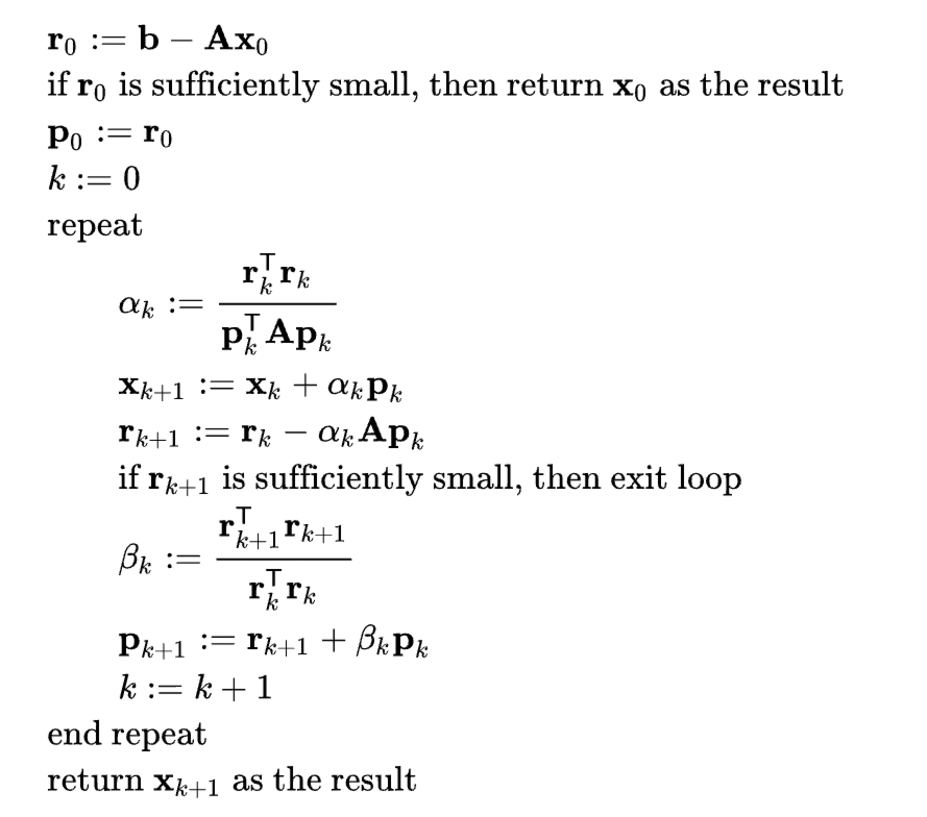
\includegraphics[width=\textwidth]{ConjGradWikipedia.pdf}
      \end{column}
      \begin{column}{0.5\textwidth}
        {\miniscule
\begin{verbatim}
  void operator()(LinearOperatorBase<Field> &Linop, const Field &src, Field &psi) 
  {
    RealD cp, c, a, d, b, ssq, qq;

    Field p(src), mmp(src), r(src);

    Linop.HermOpAndNorm(psi, mmp, d, b);
    
    r = src - mmp;
    p = r;

    a = norm2(p);
    cp = a;
    ssq = norm2(src);

    RealD rsq = Tolerance * Tolerance * ssq;

    for (int k = 1; k <= MaxIterations; k++) {
      c = cp;

      Linop.HermOp(p, mmp);

      ComplexD dc  = innerProduct(p,mmp);
      d = dc.real();
      a = c / d;

      cp = axpy_norm(r, -a, mmp, r);
      b = cp / c;

      psi = psi + a* p ;
      p   = r   + b* p ;

      if (cp <= rsq) {
        return;
      }
    }
    assert(0);
  }
  \end{verbatim}
          }
      \end{column}
      \end{columns}

  \end{frame}

  \begin{frame}[fragile]\small\frametitle{ BiCGstab }
    For Wilson Fermions, BICGstab is the fastest conventional Krylov solver
    It is suited to solving the non-Hermitian system $$ D_w \psi = b$$

    \link{https://github.com/paboyle/Grid/blob/develop/Grid/algorithms/iterative/BiCGSTAB.h}

    \href{https://en.wikipedia.org/wiki/Biconjugate_gradient_stabilized_method}
    {{\color{blue} https://en.wikipedia.org/wiki/Biconjugate\_gradient\_stabilized\_method}}
    
  \end{frame}

\begin{frame}[fragile]\small\frametitle{ Convergence rate, critical slowing down, and preconditioning}

\begin{itemize}
\item The uniformity of the Chebyshev polynomial oscillations can be used to bound convergence rate via a maximum error over the spectral range
\begin{itemize}
\item Krylov solvers can do better than this worst case bound as polynomial coefficients are selected based on the actual spectrum
\item QCD often (index theorem) has a detached number of low modes (topological nature)
\end{itemize}
\item Condition numer $$\kappa = \frac{\lambda_{\rm max}}{\lambda_{\rm min}}$$
\item Theoretical convergence factor per iteration (c.f. R-number in epidemiology!)
$$
\sigma = \frac{\sqrt{k}-1}{\sqrt{k}+1}
$$
\item In infinite volume limit spectrum is dense and the worst case is the guaranteed case
\item Empirically, the theoretical $\sigma$ governs the long tail convergence of CG in practice
\item (left) Preconditioning: changing $\kappa$ by solving a related system
$$
 P M \psi = P  b
$$
\item If the condition number of $P M$ is substantially reduced, preconditioned system converges faster
\end{itemize}


\end{frame}

\begin{frame}[fragile]\small\frametitle{ Convergence rate, critical slowing down, and preconditioning}
\begin{itemize}
\item If the condition number of $P M$ is substantially reduced, preconditioned system converges faster
\item Ideally $P$ is a cheap-to-apply \emph{approximate inverse} of M
\item Left preconditioning
$$
P M \psi = P b
$$
\item Right preconditioning 
$$
M P \psi^\prime = b ; \psi = P \psi^\prime
$$
\item Approximating $M^{-1}$ can be focussed regions of spectrum
\item Lower $\lambda_{\rm max}$
\begin{itemize}
\item Polynomial preconditioner (e.g. Chebyshev $1/x$ over high end of spectrum); reduce rate of inner-products / reductions
\item Domain decomposed smoother such Schwarz Alternating procedure : works for high end of spectrum; reduces communication and rate of inner-products / reductions
\end{itemize}
\item Raise $\lambda_{\rm min}$
\begin{itemize}
\item Deflation of low modes $P = (1 - \sum |i\rangle\langle i|) + \sum_i  \frac{|i\rangle\langle i|}{\lambda_i}  $
\item Up to rounding, deflation can be applied infrequently in CG due to orthogonal search sequence
\end{itemize}
\end{itemize}
\end{frame}


\begin{frame}[fragile]\small\frametitle{ Schur decomposition}

\link{https://github.com/paboyle/Grid/blob/develop/Grid/algorithms/iterative/SchurRedBlack.h}

A matrix can be LDU factorised as follows. Each of $A, B, C$ or $D$ can themselves be sub-matrices
\begin{equation}
\left(
\begin{array}{cc}
A & B \\
C & D
\end{array}
\right)
= 
\left(
\begin{array}{cc}
1  &   0 \\
C A^{-1}  & 1
\end{array}
\right)
\left(
\begin{array}{cc}
A & 0\\
0 & D - C A^{-1} B
\end{array}
\right)
\left(
\begin{array}{cc}
1 & A^{-1} B  \\
0 & 1
\end{array}
\right),
\end{equation}
where the Schur complement,
$$
S = D - C A^{-1} B.
$$

\end{frame}

\begin{frame}[fragile]\small\frametitle{ Red-Black preconditioning}

We can write the Dirac operator in terms of even and odd lattice sites and perform an LDU decomposition:
\begin{equation}
M = \left(
\begin{array}{cc}
M_{ee} & M_{eo} \\
M_{oe} & M_{oo}
\end{array}
\right)
= 
\left(
\begin{array}{cc}
1  &  0 \\
M_{oe} M_{ee}^{-1}  & 1
\end{array}
\right)
\left(
\begin{array}{cc}
M_{ee} & 0\\
0 & M_{oo} - M_{oe}M_{ee}^{-1} M_{eo}
\end{array}
\right)
\left(
\begin{array}{cc}
1 &  M_{ee}^{-1}M_{eo}\\
0  & 1
\end{array}
\right),
\end{equation}
where the Schur complement, is written as $M_{pc} = M_{oo} - M_{oe}M_{ee}^{-1} M_{eo}$.

\begin{itemize}
  \item For Wilson Fermions the $M_{ee}$ is proportional to the identity.
  \item For DWF and Wilson Clover Fermions the terms are non-trivial.
  \item For the Wilson Clover term $M_{ee}$ depends on the gauge fields.
  \item For DWF $M_{ee}$ is independent of the gauge fields.
\end{itemize}

$U$ and $L$ have determinant 1 and are trivially invertible:
$$
L^{-1} = 
\left(
\begin{array}{cc}
1  &  0 \\
- M_{oe} M_{ee}^{-1}  & 1
\end{array}
\right)
\quad\quad ; \quad \quad 
U^{-1} = 
\left(
\begin{array}{cc}
1 & - M_{ee}^{-1}M_{eo}\\
0  & 1
\end{array}
\right)
$$
For the odd checkerboard, $M\psi = \eta$ becomes
$$
 M_{pc} \psi_o = \eta^\prime_o = (L^{-1} \eta)_o = \eta_o - M_{oe} M_{ee}^{-1} \eta_e
$$
The even checkerboard solution can be inferred via 
$$
M_{ee} \psi_e + M_{eo} \psi_o = \eta_e \Rightarrow \psi_e = M_{ee}^{-1} (\eta_e - M_{eo} \psi_o)
$$
\begin{center}
\fbox{$M_{pc}$ (empirically) better conditioned than $M$: red black solvers converge O(3x) faster}
\end{center}
\end{frame}

\begin{frame}[fragile]\small\frametitle{Checkerboarding}

  \begin{itemize}
  \item Lattice  QCD makes use of red-black preconditioning in many algorithms
  \item Support for checkerboarded grids is required
  \begin{itemize}
  \item e.g. a field that lives only on the white or black sites of a chessboard
  \item Shifting a ``black'' field by one site produces a white field and vice versa\\ Indexing and neighbour indexing is complicated by this
  \item Stencil operators work with checkerboarded grids
  \end{itemize}
  \end{itemize}
\begin{center}
  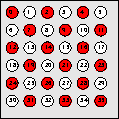
\includegraphics[height=0.2\textheight]{cb.pdf}
  \begin{minipage}{0.1\textwidth}{\hspace{0.25\textwidth}$\longleftrightarrow$\vspace{0.15\textheight}}\end{minipage}
    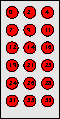
\includegraphics[height=0.2\textheight]{cbeven.pdf}
  \begin{minipage}{0.06\textwidth}{\hspace{0.25\textwidth}$+$\vspace{0.15\textheight}}\end{minipage}
    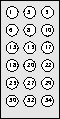
\includegraphics[height=0.2\textheight]{cbodd.pdf}
\end{center}
\begin{itemize}
\item Checkerboarded Grid objects can have arbitrary subset of dimensions involved in checkerboarding
\item Dimension ``collapsed'' can be selected (typically x-direction)
\item Natural support for 4d and 5d checkerboarded chiral fermions  
\begin{itemize}
  \item Neighbour indexing is integer heavy divide/modulo arithmetic
  \item Precompute neighbour tables in high performance Stencil objects
  \item Calculate dynamically for Cshift, looping over planes
\end{itemize}
\end{itemize}
\end{frame}

  \begin{frame}[fragile]\small\frametitle{ Eigensolvers}
\begin{itemize}
\item   The Lanczos sequence can also be used to solve for eigenvectors, known as the Lanczos algorithm.
\item   Grid has a Chebyshev polynomial preconditioned Lanczos algorithm:
\end{itemize}
\link{https://github.com/paboyle/Grid/blob/develop/Grid/algorithms/iterative/ImplicitlyRestartedLanczos.h}
\begin{itemize}
\item We will not discuss Lanczos in detail: it is used to produce the lowest lying eigenvectors of the Dirac operator
\item These can be handled exactly, and removed from the problem to eliminate critical slowing down
\item Deflation of low modes $G = \sum_i  \frac{|i\rangle\langle i|}{\lambda_i}  $ can be used as a guess.\\
\begin{itemize}
\item      These will not reenter the Krylov space other than through:
\item a) Rounding errors
\item b) Imprecision in the eigenvectors/eigenvalues
\end{itemize}
\end{itemize}
  \end{frame}


\begin{frame}[fragile]\small\frametitle{ Exercise}

\begin{itemize}
\item Write a conjugate gradients algorithm to invert the (massive) Laplacian
\begin{itemize}
\item Introduce a small mass $m^2$ to the Laplacian example in Lecture 1 to regulate the spectrum.
\end{itemize}
\href{https://github.com/paboyle/Grid/blob/develop/examples/Example_Laplacian_solver.cc}
     {\color{blue} https://github.com/paboyle/Grid/blob/develop/examples/Example\_Laplacian\_solver.cc}
\item Extension:
\begin{itemize}
\item Verify the results on the free field via Fourier methods
\item Check gauge covariance
\end{itemize}
\end{itemize}

\end{frame}




\end{document}



